% ------------------------------------------------------------------------------
% TYPO3 CMS 8.3 - What's New - Chapter "In-Depth Changes" (English Version)
%
% @author	Patrick Lobacher <patrick@lobacher.de> and Michael Schams <schams.net>
% @license	Creative Commons BY-NC-SA 3.0
% @link		http://typo3.org/download/release-notes/whats-new/
% @language	English
% ------------------------------------------------------------------------------
% LTXE-CHAPTER-UID:		5ebcecbe-66abfa57-cf38bc00-aa637965
% LTXE-CHAPTER-NAME:	In-Depth Changes
% ------------------------------------------------------------------------------

\section{Systeemwijzigingen}
\begin{frame}[fragile]
	\frametitle{Systeemwijzigingen}

	\begin{center}\huge{Hoofdstuk 3:}\end{center}
	\begin{center}\huge{\color{typo3darkgrey}\textbf{Systeemwijzigingen}}\end{center}

\end{frame}

% ------------------------------------------------------------------------------
% LTXE-SLIDE-START
% LTXE-SLIDE-UID:		8f0257d6-851ec009-500b4955-aee6ae90
% LTXE-SLIDE-ORIGIN:	bd33b29d-c20d1765-f923f78e-43bfb0bf English
% LTXE-SLIDE-TITLE:		Feature #74365: Add Linkservice for Unified Referencing Syntax (1)
% LTXE-SLIDE-REFERENCE:	Feature-74365-LinkServiceForUnifiedReferencingSyntax.rst
% ------------------------------------------------------------------------------
\begin{frame}[fragile]
	\frametitle{Systeemwijzigingen}
	\framesubtitle{Linkservice voor standaard verwijzingssyntax (1)}

	\begin{itemize}

		\item Binnen TYPO3 werd er op verschillende manieren verwezen naar bronnnen.

		\item TYPO3 ondersteunt nu een moderne, toekomstzekere manier om naar bronnen te verwijzen met een uitbreidbare en
			duidelijk syntax die eenvoudig te begrijpen is.

		\item De volgende pagina's leggen de syntax uit met de volgende, simpele link naar een pagina:

			\begin{lstlisting}
				t3://page?uid=13&campaignCode=ABC123
			\end{lstlisting}

	\end{itemize}

\end{frame}

% ------------------------------------------------------------------------------
% LTXE-SLIDE-START
% LTXE-SLIDE-UID:		731c8ef3-79b59a31-1e419214-57f1b175
% LTXE-SLIDE-ORIGIN:	95f9a663-ea2155a1-5635728b-77a8995c English
% LTXE-SLIDE-TITLE:		Feature #74365: Add Linkservice for Unified Referencing Syntax (2)
% LTXE-SLIDE-REFERENCE:	Feature-74365-LinkServiceForUnifiedReferencingSyntax.rst
% ------------------------------------------------------------------------------
\begin{frame}[fragile]
	\frametitle{Systeemwijzigingen}
	\framesubtitle{Linkservice voor standaard verwijzingssyntax (2)}

	\begin{itemize}

		\item De syntax bestaat uit drie delen:

			\begin{itemize}

				\item Namespace (\texttt{t3://})\newline
		   			De namespace is altijd \texttt{t3://} om te zorgen dat de "LinkService" wordt uitgevoerd voor deze URN.
					\newline
				\item Sleutel van bronbehandelaar (\texttt{page})\newline
   					De sleutel van de bronbehandelaar is een lijst van behandelaars die beschikbaar zijn in TYPO3.
   					Momenteel bestaan de volgende behandelaars: \texttt{page}, \texttt{file} en \texttt{folder}.\newline
					Meer sleutels kunnen geconfigureerd worden in een associatieve array waarbij de index de behandelaarsleutel is
					en de waarde een klasse is die de LinkHandlerInterface implementeert:\newline
					\texttt{\$TYPO3\_CONF\_VARS['SYS']['linkHandler']}

			\end{itemize}

	\end{itemize}

\end{frame}

% ------------------------------------------------------------------------------
% LTXE-SLIDE-START
% LTXE-SLIDE-UID:		c0b0ca2b-6fb304a7-8ae4e744-f50d12eb
% LTXE-SLIDE-ORIGIN:	77a8995c-ea2155a1-95f9a663-5635728b English
% LTXE-SLIDE-TITLE:		Feature #74365: Add Linkservice for Unified Referencing Syntax (3)
% LTXE-SLIDE-REFERENCE:	Feature-74365-LinkServiceForUnifiedReferencingSyntax.rst
% ------------------------------------------------------------------------------
\begin{frame}[fragile]
	\frametitle{Systeemwijzigingen}
	\framesubtitle{Linkservice voor standaard verwijzingssyntax (3)}

	\begin{itemize}

		\item ...en deel 3:

			\begin{itemize}

				\item Bronparameters (\texttt{?uid=13\&campaignCode=ABC123})\newline
					Dit zijn de specifieke identificatieparameters die gebruikt worden door een behandelaar.
					Let op dat deze extra parameters kunnen bevatten om het gedrag van een behandelaar te bepalen.

			\end{itemize}

	\end{itemize}

\end{frame}

% ------------------------------------------------------------------------------
% LTXE-SLIDE-START
% LTXE-SLIDE-UID:		53be962f-37345eaf-48065b75-f68f81ef
% LTXE-SLIDE-ORIGIN:	af8e73a4-2b315873-bb6e55e4-c0cd82b5 English
% LTXE-SLIDE-TITLE:		#76008 and #76458: DebuggerUtility::var_dump (1)
% LTXE-SLIDE-REFERENCE:	Feature-76008-PropertyVisibilityToDebuggerUtilityvar_dump.rst
% LTXE-SLIDE-REFERENCE:	Feature-76458-LetDebuggerUtilityRenderClosures.rst
% ------------------------------------------------------------------------------
\begin{frame}[fragile]
	\frametitle{Systeemwijzigingen}
	\framesubtitle{\texttt{DebuggerUtility::var\_dump} (1)}

	\begin{itemize}

		\item Informatie over de zichtbaarheid van een eigenschap is toegevoegd aan \texttt{DebuggerUtility::var\_dump()}
			\newline
			voor elke eigenschap van een object in de uitvoer

		\item Als een closure onderdeel is van het object dat gedebugd wordt, dan wordt de broncode hiervan ook afgebeeld

	\end{itemize}

	\tabto{0.75cm}\textit{Zie voorbeeld op de volgende pagina}

\end{frame}

% ------------------------------------------------------------------------------
% LTXE-SLIDE-START
% LTXE-SLIDE-UID:		7be78459-f3f8e020-20d58135-22f08f31
% LTXE-SLIDE-ORIGIN:	bb6e55e4-2b315873-c0cd82b5-af8e73a4 English
% LTXE-SLIDE-TITLE:		#76008 and #76458: DebuggerUtility::var_dump (2)
% LTXE-SLIDE-REFERENCE:	Feature-76008-PropertyVisibilityToDebuggerUtilityvar_dump.rst
% LTXE-SLIDE-REFERENCE:	Feature-76458-LetDebuggerUtilityRenderClosures.rst
% ------------------------------------------------------------------------------
\begin{frame}[fragile]
	\frametitle{Systeemwijzigingen}
	\framesubtitle{\texttt{DebuggerUtility::var\_dump} (2)}

	\begin{figure}
		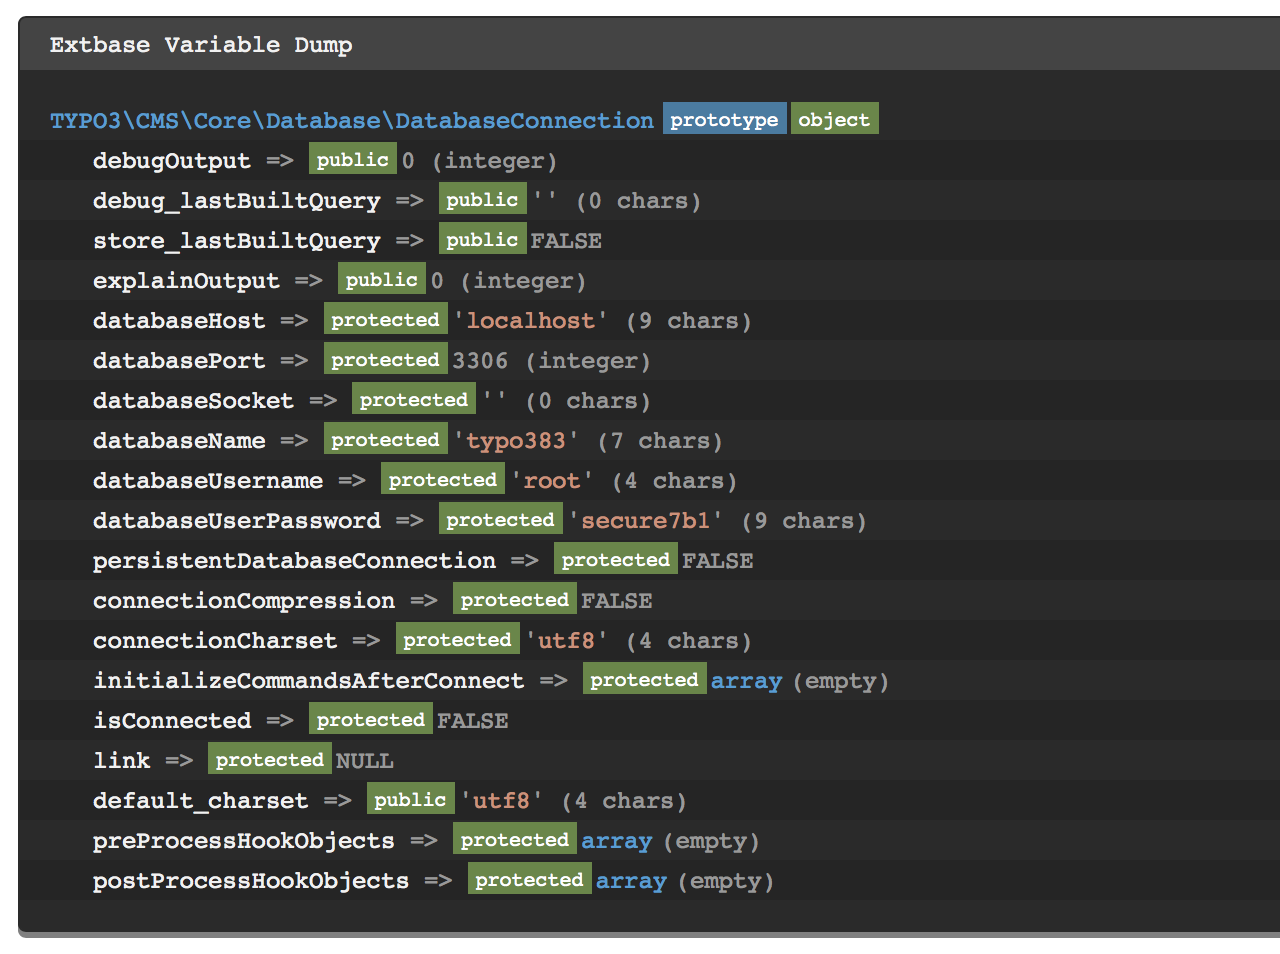
\includegraphics[width=0.65\linewidth]{InDepthChanges/76008.png}
	\end{figure}

\end{frame}

% ------------------------------------------------------------------------------
% LTXE-SLIDE-START
% LTXE-SLIDE-UID:		03142a9f-4c13c26c-95631634-ac7c3a49
% LTXE-SLIDE-ORIGIN:	2b74180d-e68ba0c2-8826a2cf-8498f977 English
% LTXE-SLIDE-TITLE:		!Breaking: #73461 - Import module disabled for non admin users
% LTXE-SLIDE-REFERENCE:	!Breaking-73461-ImportModuleDisabledForNonAdminUsers.rst
% ------------------------------------------------------------------------------
\begin{frame}[fragile]
	\frametitle{Systeemwijzigingen}
	\framesubtitle{Module importeren uitgeschakeld voor niet-admin-gebruikers}

	\begin{itemize}

		\item De importmodule van \texttt{EXT:impexp} is nu standaard uitgeschakeld voor niet-admin-gebruikers

		\item Voor niet-admin-gebruikers die de functionaliteit nodig hebben kan de volgende User TSconfig optie ingesteld
			worden:\newline
			\texttt{options.impexp.enableImportForNonAdminUser = 1}

			\vspace{0.5cm}

			\begingroup
				\color{typo3red}
				Waarschuwing: dit kan een beveiligingsprobleem worden in TYPO3 versies 6.2 en 7.6
				en zou alleen ingeschakeld moeten worden voor \textit{betrouwbare} backendgebruikers.
			\endgroup

	\end{itemize}

\end{frame}

% ------------------------------------------------------------------------------
% LTXE-SLIDE-START
% LTXE-SLIDE-UID:		47039520-2418c2c0-a292e988-a3aadbf0
% LTXE-SLIDE-ORIGIN:	bac423cc-ba00db30-e1538b7f-25749380 English
% LTXE-SLIDE-TITLE:		Hooks and Signals (1)
% LTXE-SLIDE-REFERENCE:	!Feature-76209-HookToRegisterCustomResultBrowsersInAbstractPlugin.rst
% ------------------------------------------------------------------------------
\begin{frame}[fragile]
	\frametitle{Systeemwijzigingen}
	\framesubtitle{Hooks en Signals (1)}

	% decrease font size for code listing
	\lstset{basicstyle=\tiny\ttfamily}

	\begin{itemize}

		\item Er is een nieuwe hook voor het registreren van eigen implementaties van de paginator

		\item Hiermee kan de standaard paginator van \texttt{AbstractPlugin::pi\_list\_browseresults()}
			overschreven worden voor alle of slechts specifieke extensies

		\item De hook kan geregistreerd worden in \texttt{ext\_localconf.php}:

			\begin{lstlisting}
				$GLOBALS['TYPO3_CONF_VARS']['SC_OPTIONS']
				  [\TYPO3\CMS\Frontend\Plugin\AbstractPlugin::class]['pi_list_browseresults'][1463475262] =
				  \Vendor\ExtensionKey\Hook\ResultBrowserHook::class
			\end{lstlisting}

	\end{itemize}

\end{frame}


% ------------------------------------------------------------------------------
% LTXE-SLIDE-START
% LTXE-SLIDE-UID:		33e80bc4-d3142e31-428ca90e-9bb9890f
% LTXE-SLIDE-ORIGIN:	82c70aee-3b375252-6cac0ad6-b385b95f English
% LTXE-SLIDE-TITLE:		Hooks and Signals (2)
% LTXE-SLIDE-REFERENCE:	!Feature-76259-IntroduceBuildQueryParametersPostProcessHook.rst
% ------------------------------------------------------------------------------
\begin{frame}[fragile]
	\frametitle{Systeemwijzigingen}
	\framesubtitle{Hooks en Signals (2)}

	% decrease font size for code listing
	\lstset{basicstyle=\tiny\ttfamily}

	\begin{itemize}

		\item Met de migratie naar Doctrine is de hook \texttt{buildQueryParameters} toegevoegd in de klasse
			\texttt{DatabaseRecordList}.

		\item Deze vervangt de hook \texttt{makeQueryArray} uit de verouderde methode
			\texttt{AbstractDatabaseRecordList::makeQueryArray}.

		\item Met de nieuwe hook kunnen de parameters gewijzigd worden die gebruikt worden voor de databasequery
			voor het afbeelden van de lijst met records.

		\item De hook kan geregistreerd worden in \texttt{ext\_localconf.php}:

			\begin{lstlisting}
				$GLOBALS['TYPO3_CONF_VARS']['SC_OPTIONS']
				  [\TYPO3\CMS\Recordlist\RecordList\DatabaseRecordList::class]['buildQueryParameters'][]
			\end{lstlisting}

		\item ...en implementeert de publieke methode \texttt{buildQueryParametersPostProcess}

	\end{itemize}

\end{frame}

% ------------------------------------------------------------------------------
% LTXE-SLIDE-START
% LTXE-SLIDE-UID:		523dacba-cd643659-e5d69af8-9de1f03d
% LTXE-SLIDE-ORIGIN:	73d888ce-a14c0f6a-d4dec5fb-f7368bb6 English
% LTXE-SLIDE-TITLE:		!Breaking: #76108 - Replace ExtJS category tree with D3 and SVG
% LTXE-SLIDE-TITLE:		!Feature: #77349 - Additional locations for extension icons
% LTXE-SLIDE-TITLE:		!Feature: #77481 - Add possibility to define a favicon for the backend
% LTXE-SLIDE-REFERENCE:	!Breaking-76108-ReplaceExtJSCategoryTreeWithD3AndSVG.rst
% LTXE-SLIDE-REFERENCE:	!Feature-77349-AdditionalLocationsForExtensionIcons.rst
% LTXE-SLIDE-REFERENCE:	!Feature-77481-AddPossibilityToDefineAFaviconForTheBackend.rst
% ------------------------------------------------------------------------------
\begin{frame}[fragile]
	\frametitle{Systeemwijzigingen}
	\framesubtitle{Miscellaneous}

	\begin{itemize}

		\item SVGs en D3 rendering

			\begin{itemize}
				\item Als onderdeel van het verwijderen van ExtJS is de boom voor de formulieren opnieuw gebouwd
				\item Het renderen is gebaseerd op SVG's en D3 waardoor prestaties significant verbeteren
				\item Het opnieuw bouwen van de paginaboom op deze wijze is gepland voor de nabije toekomst
			\end{itemize}

		\item Iconen voor extensies kunnen opgeslagen worden in de directory:\newline
			\small
				\texttt{Resources/Public/Icons/<bestandsnaam>}
				(<bestandsnaam> kan zijn: \texttt{Extension.png}, \texttt{Extension.svg} or \texttt{Extension.gif})
			\normalsize

		\item De nieuwe opties \texttt{backendFavicon} in de configuratie van Extensiebeheer maakt het mogelijk om het favicon
			van de backend te wijzigen.

	\end{itemize}

\end{frame}

% ------------------------------------------------------------------------------
